\documentclass{article}
\usepackage[utf8]{inputenc}

\usepackage{graphicx,caption}
\graphicspath{ {./images/} }
\usepackage{float}
\usepackage{caption}
\usepackage{subcaption}
\usepackage[unicode]{hyperref}
\usepackage{amsmath}
\usepackage[shortlabels]{enumitem}

\usepackage{listings}
\usepackage{xcolor}
\definecolor{codegreen}{rgb}{0,0.6,0}
\definecolor{codegray}{rgb}{0.5,0.5,0.5}
\definecolor{codepurple}{rgb}{0.58,0,0.82}
\definecolor{backcolour}{rgb}{0.95,0.95,0.92}
 \lstdefinestyle{mystyle}{
    backgroundcolor=\color{backcolour},   
    commentstyle=\color{codegreen},
    keywordstyle=\color{black},
    numberstyle=\tiny\color{codegray},
    stringstyle=\color{codepurple},
    basicstyle=\ttfamily\footnotesize,
    breakatwhitespace=false,         
    breaklines=true,                 
    captionpos=b,                    
    keepspaces=true,                 
    numbers=left,                    
    numbersep=5pt,                  
    showspaces=false,                
    showstringspaces=false,
    showtabs=false,                  
    tabsize=2
}
\lstset{style=mystyle}

\title{Homework 6 - Theory/Laboratory}
\author{Dainese Fabio, 857661}
\date{April 12, 2020}

\begin{document}

\maketitle

\section{Load, Visualize and Analyse Network Data}
    After loaded the '\textit{VIPD.mat}' file and generated the relative sub-graph without isolated nodes starting from the first 2 columns (\textit{source, target}), we have obtained the following results:
    
    \begin{figure}[H]
            \centering
            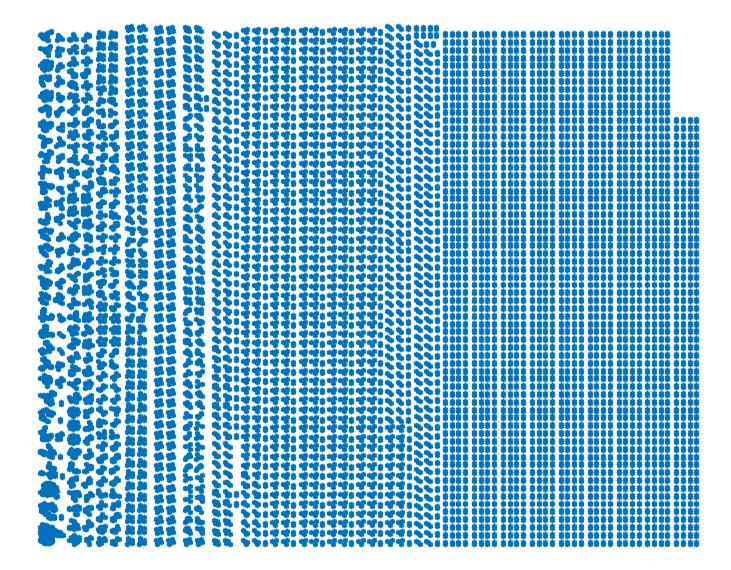
\includegraphics[width=\textwidth]{1.png}
            \caption{Plot of the sub-graph using the '\textit{force}' layout}
            \label{fig:figure-1}
    \end{figure}
    
    \begin{figure}[H]
            \centering
            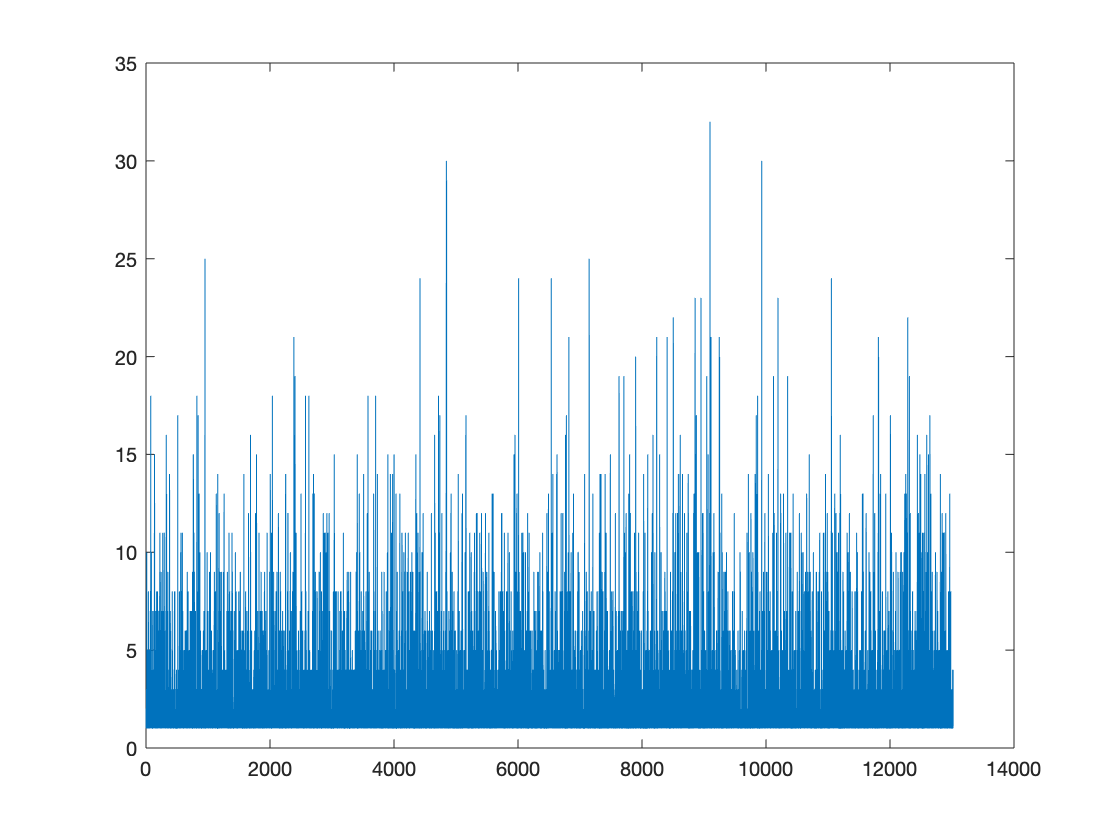
\includegraphics[width=0.9\textwidth]{2.0.png}
            \caption{Plot of the degree distribution of the sub-graph (unsorted)}
            \label{fig:figure-2.0}
    \end{figure}
    \begin{figure}[H]
            \centering
            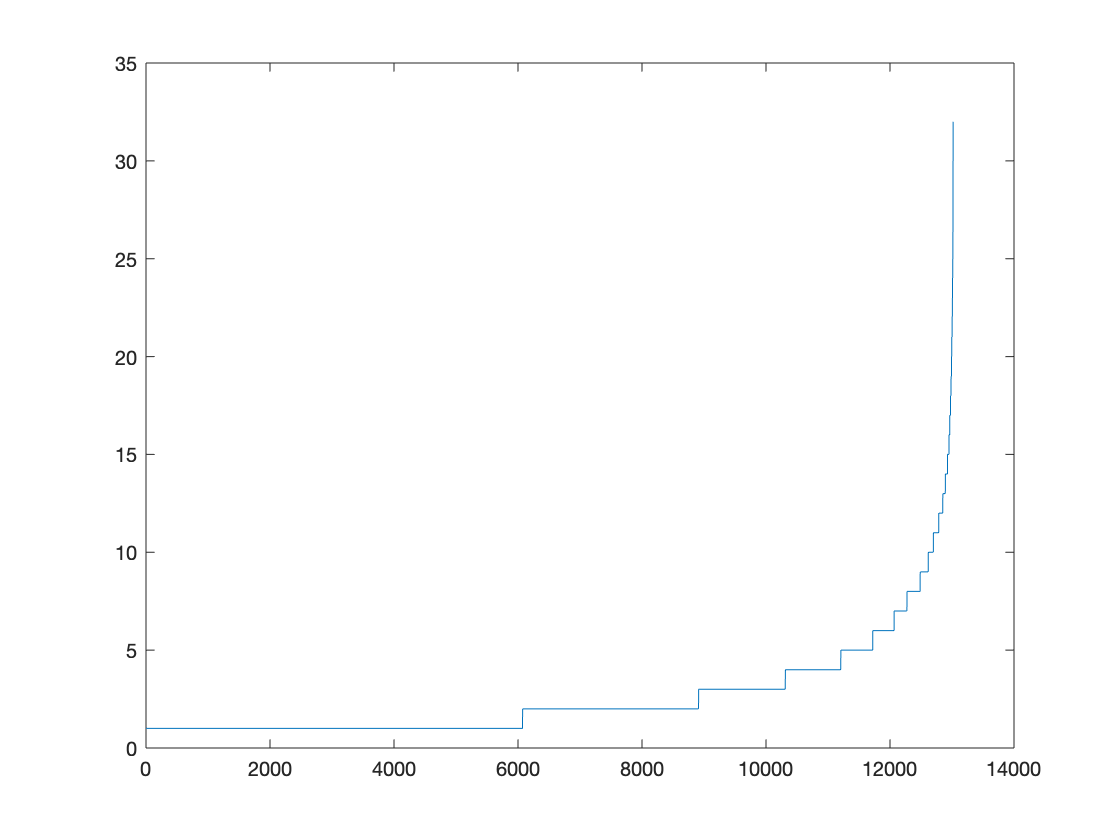
\includegraphics[width=0.9\textwidth]{2.1.png}
            \caption{Plot of the degree distribution of the sub-graph (sorted)}
            \label{fig:figure-2.1}
    \end{figure}
    
    \begin{itemize}
        \item The average degree is \(2.595591\)
        \item The average clustering coefficient is \(0.421364\)
        \item The average path length is \(0.034427\).\newline
        
        \par\noindent To precise that it has been used the following formula to calculate the APL:
        \[APL(G)=\frac{1}{n \cdot (n-1)} \sum_{i \neq j}d(v_{i},v_{j})\]
        where \(n\) is the number of nodes in the graph \(G\) and also assume that \(d(v_{1},v_{2})=0\) if \(v_{2}\) cannot be reached from \(v_{1}\).\newline
        
        \par\noindent This clarification is due since the MatLab function '\textit{distances(G)}' doesn't put \(0\) whenever a specific node cannot be reached, instead it puts '\textit{Infinite}' (so using '\textit{mean(distances(G))}' did returned the expected value).
        
        \item The number of nodes of the sub-graph are \(13019\)
    \end{itemize}
    \bigskip
    \par\noindent These previous results have been calculated using the following \textit{MatLab} script:
    \newline
    \begin{lstlisting}[language=Matlab]
clear all;
clc;

% =================================================================
% ====================== 1 - Load the data ========================
% =================================================================

load VIPD.mat;

s = table2array(VIPDedgelist(:,1));
t = table2array(VIPDedgelist(:,2));

G = graph(s,t,[],max(s));

% =================================================================
% =================== 2 - Generate a subgraph =====================
% =================================================================

cnt = 'degree';
d = centrality(G,cnt);

G_New = subgraph(G,d>=1);

% =================================================================
% =================== 3 - Plot the sub-graph ======================
% =================================================================

figure(1)
plot(G_New,'Layout','force','iterations',10);

% =================================================================
% ============== 4 - Plot the degree distribution =================
% =================================================================

deg = degree(G_New);

figure(2)
plot(deg)
plot(sort(deg));

% =================================================================
% ================ 5 - Find the average degree ====================
% =================================================================

fprintf('%f \n',mean(deg));

% =================================================================
% ========= 6 - Find the average clustering coefficient ===========
% =================================================================

cc = clustering_coef_bu(G_New.adjacency);
fprintf('%f \n',mean(cc));

% =================================================================
% ============== 7 - Find the average path length =================
% =================================================================

pl = distances(G_New);
% Replace all the 'Infinite' with '0' in the matrix
pl(~isfinite(pl)) = 0;
n = numnodes(G_New);
fprintf('%f \n',(sum(pl,'all')/(n*(n-1))));

% =================================================================
% ========== 8 - Find the number of nodes of the graph ============
% =================================================================

fprintf('%d \n',numnodes(G_New));
\end{lstlisting}

\section{Calibrate Random Network Models}
The value of the parameters of the different models (\textit{ER,WS,BA}) which make the average node degree of each of them close to the one of the interlocking directorate (ID) network are:

\begin{itemize}
    \item \textbf{ER model}  \(G_{ER}(n,p)\) \newline
    
    \par\noindent With the number of nodes equals to \(n = 13019\) (the same of the ID sub-graph) and the edge probability equals to \(p=0.0002\), we have an average node degree of \(2.5941\).
    
    \item \textbf{WS model}  \(G_{WS}(n,K,p)\) \newline
    
    \par\noindent With the number of nodes equals to \(n = 13019\) (the same of the ID sub-graph), the number of neighbours in each side for each node equals to \(K=1\) (\(2K\) = the number of neighbours for each node = node degree) and the re-wiring probability \(q\) (in this case is indifferent the value of \(q\) since the  re-wiring procedure doesn't alter the number of edges for each node, thus also the node degree), we have an average node degree of \(2\).
    
    \item \textbf{BA model}  \(G_{BA}(n,m,m_{0})\) (with \(1 < m < m_{0}\)) \newline
    
    \par\noindent With the number of nodes equals to \(n = 13019\) (the same of the ID sub-graph), the initial number of connected nodes equals to \(m = 1\) and the number of edges generated at each iteration \(m_{0}\) (indifferent also in this case), we have an average node degree of \(2\).
\end{itemize}

\bigskip
\noindent In the following table you can see the comparison between the three calibrated models and the ID data over some statistics:\newline
\begin{center}
    \begin{tabular}{ |c|c|c|c| } 
    \hline
    Model Name & Average CC & Average PL & Average Degree \\
    \hline
    ID sub-graph & 0.421364 & 0.034427 & 2.595591 \\
    ER & 0.000156 & 7.8931 & 2.5941 \\
    WS (\(q=0.5\)) & 0 & 22.584 & 2 \\
    BA (\(m_{0}=2\)) & 0 & 7.122 & 2 \\
    \hline
    \end{tabular}
\end{center}
\bigskip
\bigskip
    \par\noindent In the following histogram ('Figure \ref{fig:figure-3}'), you can see a direct comparison between the different models (\textit{ER,WS,BA}) and the ID data over the degree distribution.\newline
    To point out that in the plot the range of degrees have been limited up to 20 in order to understand more clearly the data (zoom in the range that contains the peaks).

    \begin{figure}[H]
            \centering
            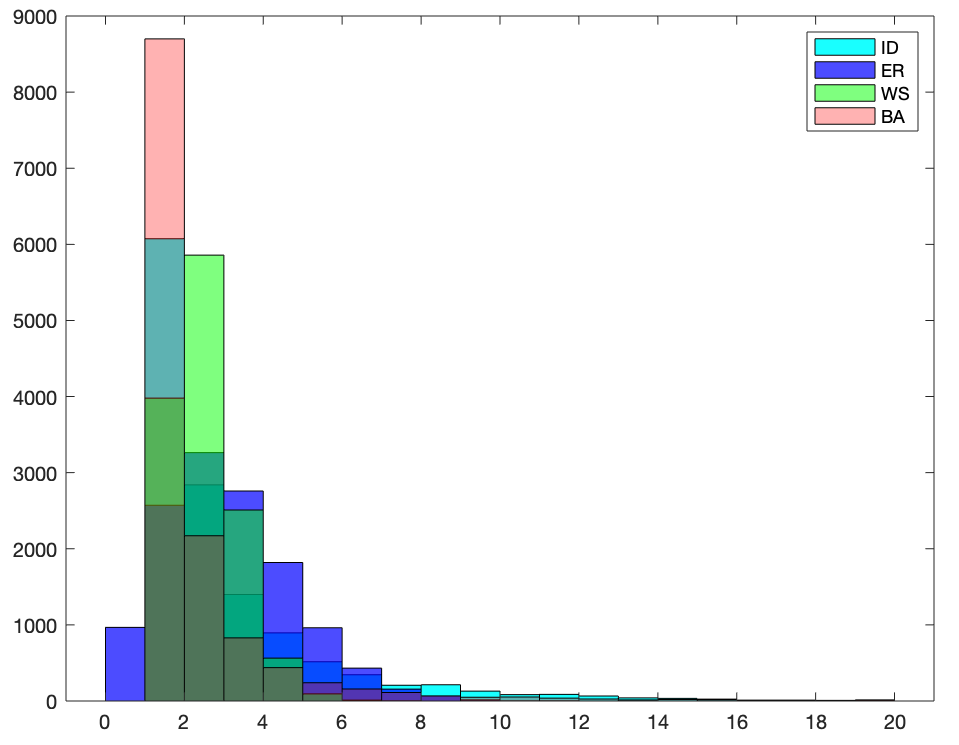
\includegraphics[width=1\textwidth]{3.png}
            \caption{The degree distribution for the models and the ID data}
            \label{fig:figure-3}
    \end{figure}
    
    \bigskip
    \bigskip
    
    \par\noindent The best model for the ID network is the BA (\textit{Albert-Barabasi}) one, since it's the most similar starting from the previous experiment results and clearly visible by looking its degree distribution that fits the original one (see the next 2 plots).
    
    \begin{figure}[H]
        \centering
        \begin{minipage}[b]{0.48\textwidth}
            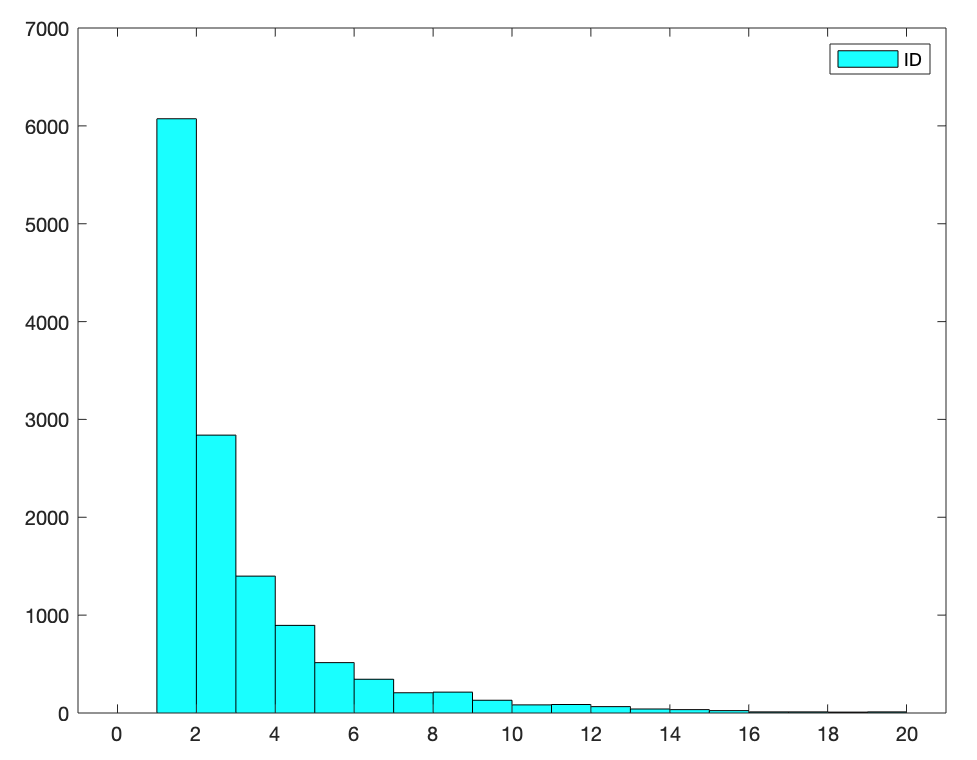
\includegraphics[width=\textwidth]{ID.png}
            \subcaption{Isolated zoomed degree distribution of ID}
            \label{fig:figure-4-a}
        \end{minipage}
        \hfill
        \begin{minipage}[b]{0.48\textwidth}
            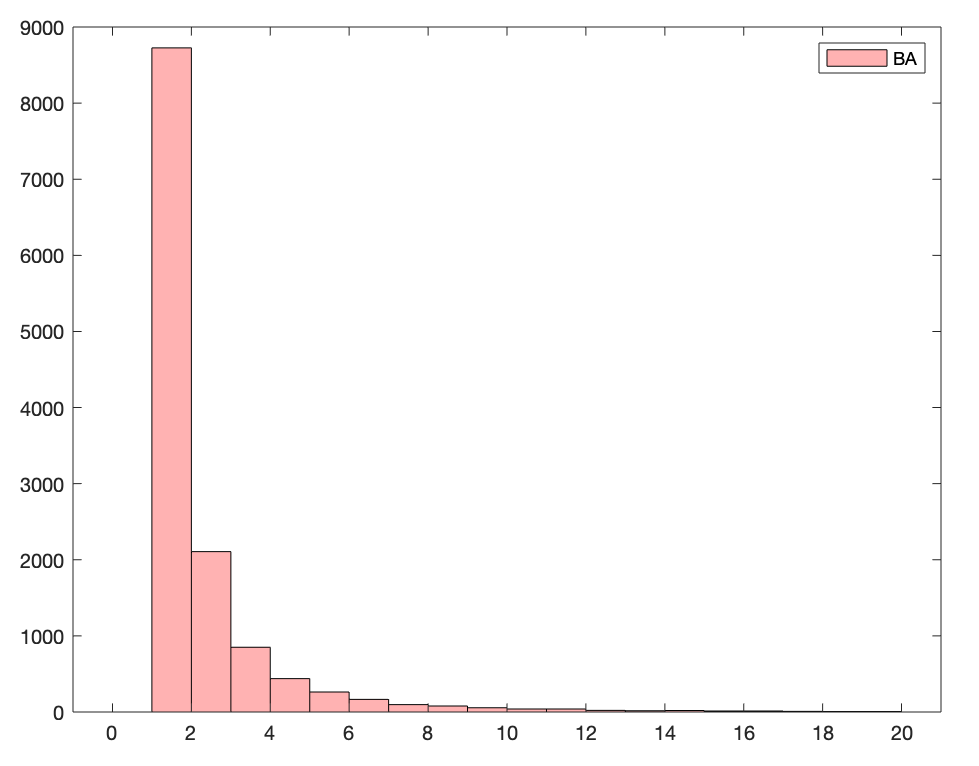
\includegraphics[width=\textwidth]{BA.png}
            \subcaption{Isolated zoomed degree distribution of BA}
            \label{fig:figure-4-b}
        \end{minipage}
        \label{fig:figure-4}
    \end{figure}

\end{document}
